\section{Inference and Experiments}

In this section, we put our skills together to analyze an A/B test. We'll use pandas, NumPy, and a couple new things.

\begin{enumerate}
    \item Use \code{statsmodels} for ordinary least squares.\footnote{You might notice \cite{vanderplas2016python} uses \code{sklearn} for linear regression. Both are good. \code{sklearn} is more ML oriented and \code{statsmodels} is more stats oriented. As an example of this difference, \code{sklearn} will apply regularization to a logistic regression by default and \code{statsmodels} won't.}
    \item Use \code{scipy} for a two-sample $t$-test.
    \item Use \code{numpy} for randomization inference/permutation tests.
\end{enumerate}


First, here's some motivation for why A/B tests are important and to create more student demand for the causal inference course I want to teach. 

\subsection{Motivation/Soapbox}
Any economic or behavioral model proposes to describe the Data Generating Process (DGP), or whatever is really driving the outcomes we see in our non-experimental data. That is, we want to work out if $X$ causes $Y$ or $X$ and $Y$ have a common cause and the association between them is spurious. What would you say if you (plausibly) analyzed data that showed people wearing winter hats are colder than people not wearing winter hats? This is all to say that questions of causality are fraught with issues of bias. Hence the oft-repeated directive \link{https://hbr.org/2021/11/leaders-stop-confusing-correlation-with-causation}{not to confuse correlation with causality}.

The diagrams below depict two different causal models. Suppose you work for a business with a subscription model. It might be Duolingo, Peloton, Netflix, etc. There is normal activity, which is simply using the product and there is social engagement, which might be liking or sharing posts on social media. A product manager might want to know the business impact of social engagement, and both models might create the same correlations between social and retention. \link{https://hbr.org/2018/12/what-great-data-analysts-do-and-why-every-organization-needs-them}{A great analyst} is sensitive to the idea that correlations are not proof of a causal relationship.

\begin{center}
    
    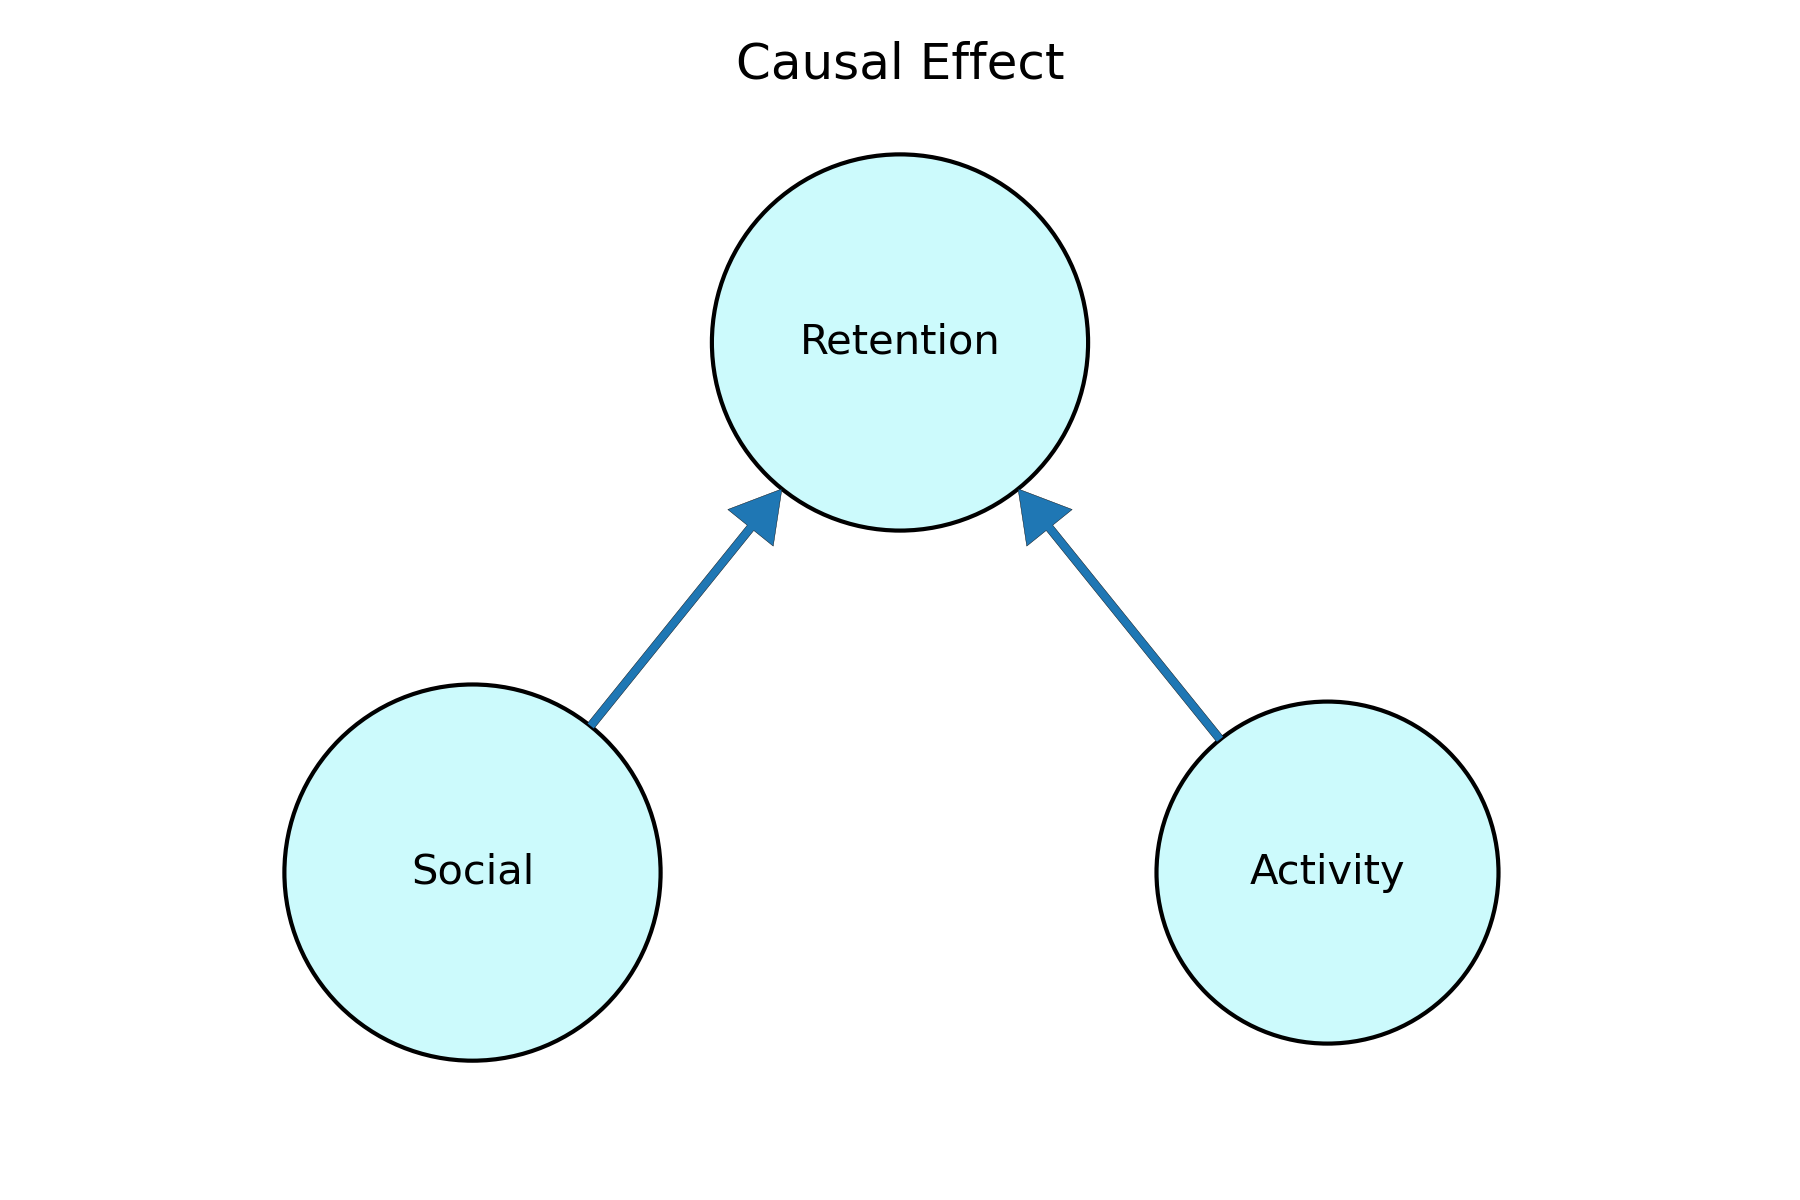
\includegraphics[width =0.48\textwidth]{images/causal1.png} 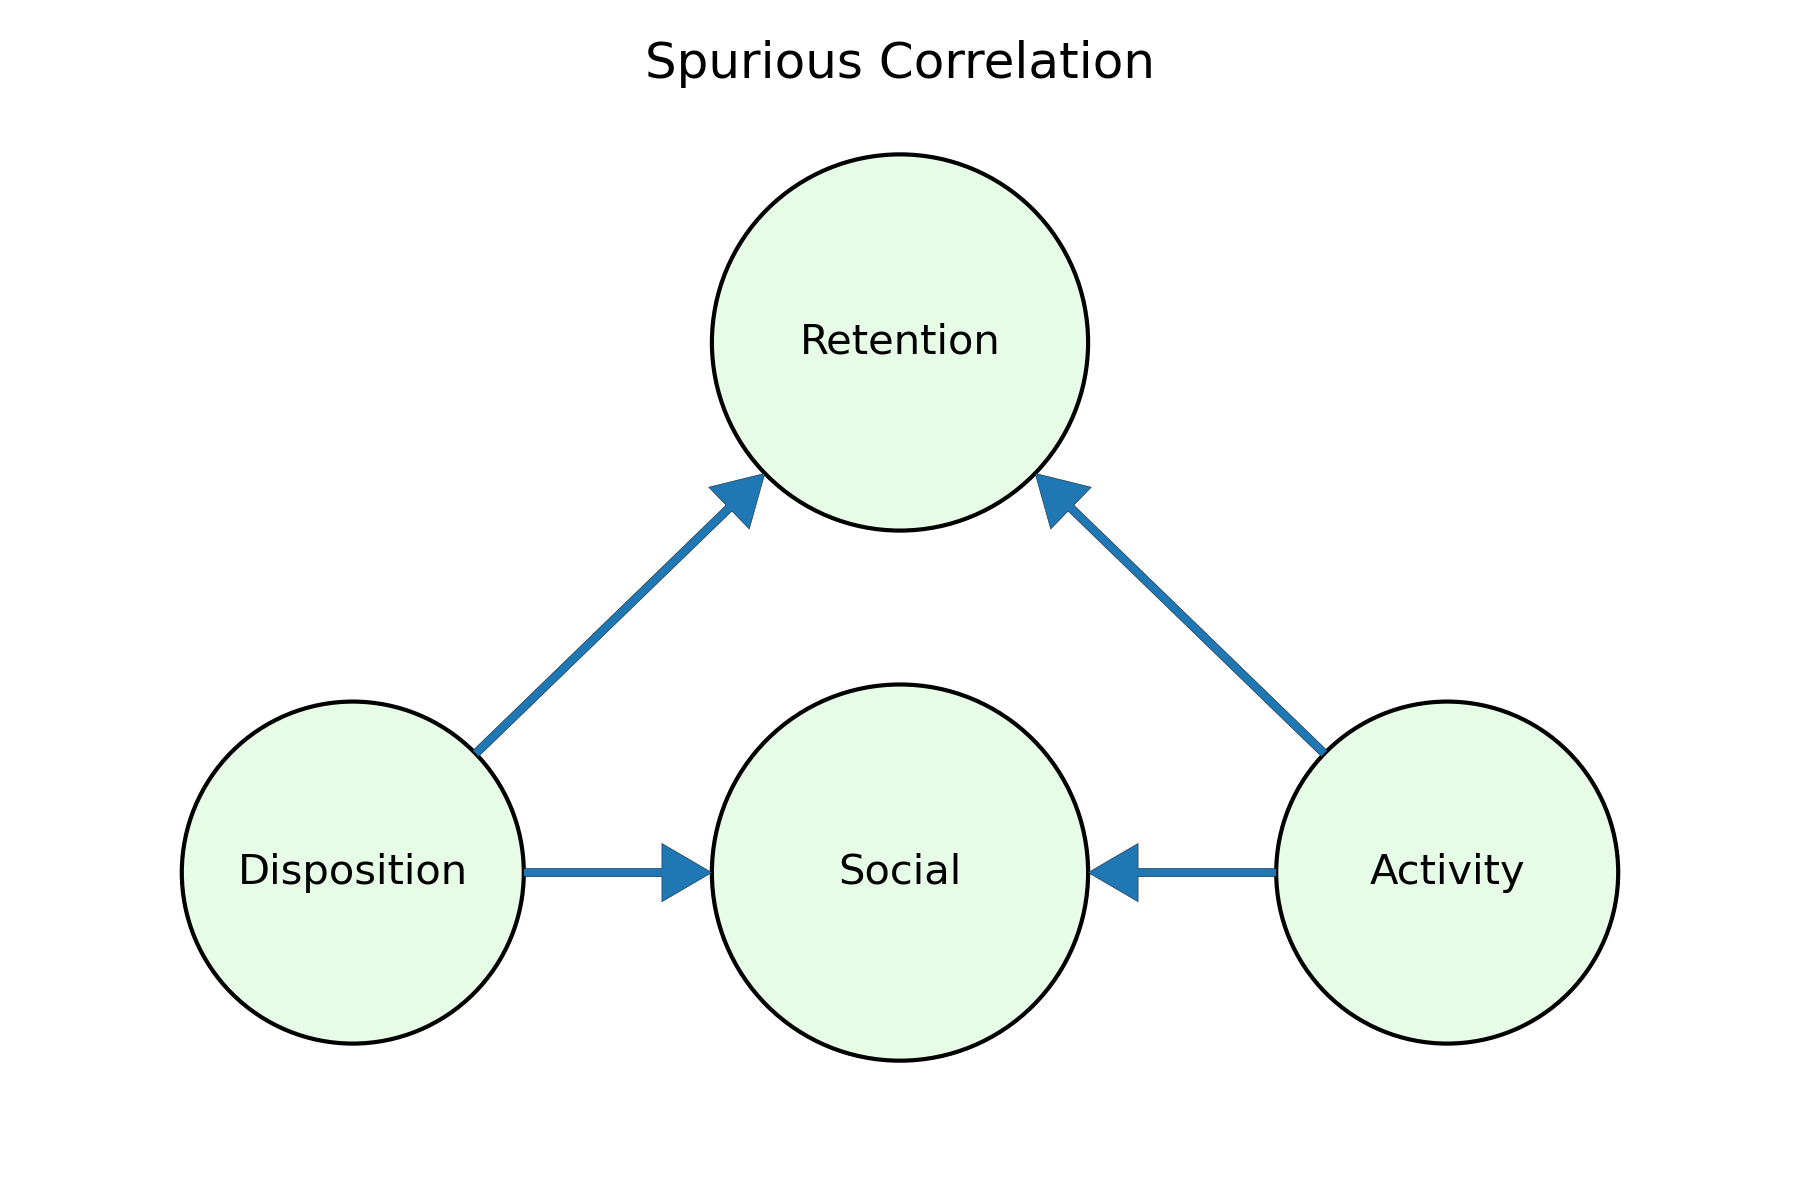
\includegraphics[width = 0.48\textwidth]{images/spurious.png}
\end{center}

On the left, social engagement has a direct effect on the retention outcome. On the right, social engagement has no effect on the retention outcome. However, as we verify in the simulation below, both can produce the same regression output. We'll use OLS for simplicity.  

We regress retention on social engagement and activity, first with data generated by the causal effect process (\code{y1}), then the spurious correlation process (\code{y2}).

\begin{lstlisting}
import statsmodels.api as sm
import pandas as pd

n = 1000
noise = np.random.normal(0, .1, size = n)

# for causal model
activity = np.random.normal(size = n)
social = np.random.normal(size = n)
intercept = np.ones(n)
disposition = np.random.normal(size = n)
social_alt = disposition + activity
    

df = pd.DataFrame()
for thing in ['activity','social','social_alt','disposition','intercept']:
    df[thing] = globals()[thing]


# Causal Model
y1 = 1*social + 1*activity + noise
X1 = df[['activity','social','intercept']]
causal_model = sm.OLS(y1, X1).fit()
print(causal_model.summary())

# Spurious Model
y2 = 2*activity + 1*disposition + noise
X2 = df[['activity','social_alt','intercept']]
spurious_model = sm.OLS(y2, X2).fit()
print(spurious_model.summary())
\end{lstlisting}

The regression output is produced below. They're the same, and that's bad. That means our simple OLS model isn't causal evidence, because the same results could be observed with a non-causal data generating process. 

\textbf{Causal effect model:}
\begin{footnotesize}
\begin{center}
\begin{tabular}{lclc}
\toprule
\textbf{Dep. Variable:}    &        y         & \textbf{  R-squared:         } &     0.995   \\
\textbf{Model:}            &       OLS        & \textbf{  Adj. R-squared:    } &     0.995   \\
\textbf{Method:}           &  Least Squares   & \textbf{  F-statistic:       } & 9.894e+04   \\
\textbf{Date:}             & Mon, 18 Apr 2022 & \textbf{  Prob (F-statistic):} &     0.00    \\
\textbf{Time:}             &     14:11:29     & \textbf{  Log-Likelihood:    } &    878.45   \\
\textbf{No. Observations:} &        1000      & \textbf{  AIC:               } &    -1751.   \\
\textbf{Df Residuals:}     &         997      & \textbf{  BIC:               } &    -1736.   \\
\textbf{Df Model:}         &           2      & \textbf{                     } &             \\
\bottomrule
\end{tabular}
\begin{tabular}{lcccccc}
                   & \textbf{coef} & \textbf{std err} & \textbf{t} & \textbf{P$> |$t$|$} & \textbf{[0.025} & \textbf{0.975]}  \\
\midrule
\textbf{activity}  &       1.0034  &        0.003     &   313.158  &         0.000        &        0.997    &        1.010     \\
\textbf{social}    &       1.0008  &        0.003     &   314.360  &         0.000        &        0.995    &        1.007     \\
\textbf{intercept} &       0.0024  &        0.003     &     0.760  &         0.447        &       -0.004    &        0.009     \\
\bottomrule
%\caption{OLS Regression Results (Causal Effect DGP)}
\end{tabular}

\end{center}
\end{footnotesize}

\textbf{Spurious correlation model:}
\begin{footnotesize}
\begin{center}
\begin{tabular}{lclc}
\toprule
\textbf{Dep. Variable:}    &        y         & \textbf{  R-squared:         } &     0.998   \\
\textbf{Model:}            &       OLS        & \textbf{  Adj. R-squared:    } &     0.998   \\
\textbf{Method:}           &  Least Squares   & \textbf{  F-statistic:       } & 2.477e+05   \\
\textbf{Date:}             & Mon, 18 Apr 2022 & \textbf{  Prob (F-statistic):} &     0.00    \\
\textbf{Time:}             &     14:09:52     & \textbf{  Log-Likelihood:    } &    878.62   \\
\textbf{No. Observations:} &        1000      & \textbf{  AIC:               } &    -1751.   \\
\textbf{Df Residuals:}     &         997      & \textbf{  BIC:               } &    -1737.   \\
\textbf{Df Model:}         &           2      & \textbf{                     } &             \\
\bottomrule
\end{tabular}
\begin{tabular}{lcccccc}
                     & \textbf{coef} & \textbf{std err} & \textbf{t} & \textbf{P$> |$t$|$} & \textbf{[0.025} & \textbf{0.975]}  \\
\midrule
\textbf{activity}    &       1.0013  &        0.005     &   220.729  &         0.000        &        0.992    &        1.010     \\
\textbf{social\_alt} &       1.0020  &        0.003     &   315.603  &         0.000        &        0.996    &        1.008     \\
\textbf{intercept}   &       0.0026  &        0.003     &     0.811  &         0.418        &       -0.004    &        0.009     \\
\bottomrule
%\caption{OLS Regression Results (Spurious Correlation DGP)}

\end{tabular}

\end{center}
\end{footnotesize}

This is frustrating, but it's why experiments hold a special place in economics and data science. For more on experiments and inference, you might check out \cite{luca2020want} for commentary on experiments and \cite{cunningham2021causal} for a text on causal inference with Python code samples. 

\subsection{Experiments}


\subsubsection{$t$-tests}
A simple A/B test is almost always analyzed by conducting a $t$-test. And typically, we have a two-sample test. For this, we can use \link{https://scipy.org/}{SciPy} and its stats submodule. 
We'll use the \code{scipy.stats.ttest_ind()} function to run a Welch's $t$-test.


\begin{lstlisting}
import scipy.stats
import numpy as np
np.random.seed(1)

n = 1000 # observations
n_sims = 5000 # simulations
n_significant_results = 0
for _ in range(n_sims):
    
    # exactly the same!
    g1 = np.random.binomial(n = 1, p = 0.5, size = n)
    g2 = np.random.binomial(n = 1, p = 0.5, size = n)
    
    n_significant_results += 1 * (scipy.stats.ttest_ind(g1,g2).pvalue <= 0.05)
    
    
print(n_significant_results/n_sims)
\end{lstlisting}

We get false positives 5.38\% of the time. 


\subsubsection{Lady Tasting Tea}

Now, we'll move toward calculating exact $p$-values using simulations. To start, we consider the classic \link{https://en.wikipedia.org/wiki/Lady_tasting_tea}{lady tasting tea} experiment. 

Irving Fisher calculated that a random guesser could get the correct result only one time out of 70. Below, we verify this with a simulation.

\begin{lstlisting}
import numpy as np
np.random.seed(24)

# without loss of generality, let truth be...
truth = np.array([1,1,1,1, 0,0,0,0])


n = 100_000
p_value = len([x for x in range(n) if np.random.permutation(truth)[0:4].sum() == 4]) / n

print(p_value)
\end{lstlisting}

\subsubsection{Randomization Inference}

Randomization inference goes just a bit beyond what's done in the lady tasting tea example. We have a single observed treatment effect and then we simulate many more counterfactual treatment effects by permuting the treatment and control assignments. The permutations simulate the kinds of treatment effects we'd observe under the null hypotheses. If we calculate how often those treatment effects are more extreme than what we actually observed, we're left with an \emph{exact} $p$-value. 

\begin{lstlisting}
users = pd.read.read_csv('users_l12.csv')
engagement = pd.read_csv('engagement_l12.csv')

# Simulate 1000 alternate labels
for i in range(1000):
    users['alt{}'.format(i)] = np.random.permutation(users.assignment)
    
df2 = engagement.merge(users, on = 'user_id')

# homework to improve this step
treatment_effects = list()
for column in [x for x in list(df2) if 'alt' in str(x)]:
    sums = df2.groupby(column).minutes_engaged.sum()
    te = sums['treatment'] - sums['control']
    treatment_effects.append(te)


# Make Plot
plt.hist(treatment_effects, bins = 30)

# actual treatment effect
grouped = df2.groupby('assignment').minutes_engaged.sum()
te_true = grouped['treatment'] - grouped['control']
plt.axvline(te_true, color = 'black')

plt.show()

abs_values = np.abs(treatment_effects)

p_value = len(abs_values[abs_values > treatment_effect()]) / 1000

print(p_value)


# compare to t-test

from scipy.stats import ttest_ind

treatment_values = df[df.assignment == 'treatment'].minutes_engaged.values
control_values = df[df.assignment == 'control'].minutes_engaged.values

test = ttest_ind(treatment_values, control_values, equal_var = False)
print('t-test p value', test.pvalue)
\end{lstlisting}